%start preamble
\documentclass[paper=a4,fontsize=11pt]{scrartcl}%kind of doc, font size, paper size
\usepackage[ngerman]{babel}%for special german letters etc			
%\usepackage{t1enc} obsolete, but some day we go back in time and could use this again
\usepackage[T1]{fontenc}%same as t1enc but better						
\usepackage[utf8]{inputenc}%utf-8 encoding, other systems could use others encoding
%\usepackage[latin9]{inputenc}			
\usepackage{amsmath}%get math done
\usepackage{amsthm}%get theorems and proofs done
\usepackage{graphicx}%get pictures & graphics done
\graphicspath{{pictures/}}%folder to stash all kind of pictures etc
\usepackage{amssymb}%symbolics for math
\usepackage{amsfonts}%extra fonts
\usepackage []{natbib}%citation style
\usepackage{caption}%captions under everything
\usepackage{listings}
\usepackage[titletoc]{appendix}
\numberwithin{equation}{section} 
\usepackage[printonlyused,withpage]{acronym}%how to handle acronyms
\usepackage{float}%for garphics and how to let them floating around in the doc
\usepackage{cclicenses}%license!
\usepackage{xcolor}%nicer colors, here used for links
\usepackage{wrapfig}%making graphics floated by text and not done by minipage
\usepackage{dsfont}
\usepackage{stmaryrd}
\usepackage{geometry}
\usepackage{hyperref}
\usepackage{fancyhdr}
\usepackage{menukeys}

%settings colors for links
\hypersetup{
    colorlinks,
    linkcolor={blue!50!black},
    citecolor={blue},
    urlcolor={blue!80!black}
}

\definecolor{pblue}{rgb}{0.13,0.13,1}
\definecolor{pgreen}{rgb}{0,0.5,0}
\definecolor{pred}{rgb}{0.9,0,0}
\definecolor{pgrey}{rgb}{0.46,0.45,0.48}

\pagestyle{fancy}
\lhead{Netzwerke Übung (SoSe 2019)}
\rhead{FB 4 -- Angewandte Informatik\\ HTW-Berlin}
\lfoot{Übungsblatt 04 -- Backbone Routing}
\cfoot{}
\fancyfoot[R]{\thepage}
\renewcommand{\headrulewidth}{0.4pt}
\renewcommand{\footrulewidth}{0.4pt}

\lstdefinestyle{Bash}{
  language=bash,
  showstringspaces=false,
  basicstyle=\small\sffamily,
  numbers=left,
  numberstyle=\tiny,
  numbersep=5pt,
  frame=trlb,
  columns=fullflexible,
  backgroundcolor=\color{gray!20},
  linewidth=0.9\linewidth,
  %xleftmargin=0.5\linewidth
}

\newlength\labelwd
\settowidth\labelwd{\bfseries viii.)}
\usepackage{tasks}
\settasks{counter-format =tsk[a].), label-format=\bfseries, label-offset=3em, label-align=right, label-width
=\labelwd, before-skip =\smallskipamount, after-item-skip=0pt}
\usepackage[inline]{enumitem}
\setlist[enumerate]{% (
labelindent = 0pt, leftmargin=*, itemsep=12pt, label={\textbf{\arabic*.)}}}

\pdfpkresolution=2400%higher resolution

%%here begins the actual document%%
\newcommand{\horrule}[1]{\rule{\linewidth}{#1}} % Create horizontal rule command with 1 argument of height

\DeclareMathOperator{\id}{id}

\begin{document}
\begin{center}
\Large{\textbf{Übungsblatt 04 -- Backbone Routing}}\\
\end{center}
Im Anschluss der letzten beiden Übungsblättern sollen Sie nun vorbereitend Ihr erstes komplexeres Netzwerk umsetzen. Die kleinen Separaten Netzwerke der letzten Laborübung sollen verknüpft werden und darüber hinaus sollen Sie für einen Anschluss an das Internet sorgen (der sogenannte Uplink). Im wesentlich wird ein solches Netzwerk auch als Backbone-Netzwerk beschrieben. Backbone-Routing wird auch an den großen Internet-Knoten umgesetzt (diese werden als Internet-Exchange-Point -- IXP bezeichnet), wie etwas dem \emph{DECIX} (\url{https://www.de-cix.net/}).\\
Wie Sie sehen, können Sie nach nur drei Übungen schon einiges an Know-How vorweisen.\\
\textbf{Inhalt:}
\begin{itemize}
	\item Routing \& Backbone-Routing 
	\item Planung eines komplexeren Netzwerkes mithilfe von Linux-Routern (Cisco gerne auf Anfrage!)
	\item Erweiterung der Tools für Netzwerkadministration
	\item \emph{ip-tables}
\end{itemize}
Hilfreiche Links (gründlich lesen, kein einfaches Copy \& Paste!):
\begin{itemize}
	\item \url{https://en.wikipedia.org/wiki/Domain_Name_System}
	\item \url{https://en.wikipedia.org/wiki/Iptables}
	\item \url{https://www.howtogeek.com/177621/the-beginners-guide-to-iptables-the-linux-firewall/}
	\item \url{https://www.digitalocean.com/community/tutorials/how-to-forward-ports-through-a-linux-gateway-with-iptables}
	\item \url{https://serverfault.com/questions/326493/basic-iptables-nat-port-forwarding}
\end{itemize}

\begin{center}\Large{\textbf{Aufgabe A -- Planung des Netzwerkes}}\end{center}\vskip0.25in
Wie in der letzten Übung arbeiten Sie zunächst in Gruppen von je vier Studierenden.\\
Bis dato sollten die Knoten Ihre beiden Netzwerke untereinander kommunizieren können. Dieser Aufbau soll nun so erweitert werden, dass Ihre Netzwerke (d.h. Ihre Bankreihe) mit den Rechnern der anderen Bankreihe kommunizieren können. Im wesentlichen kennen Sie also schon den Aufbau, Ihr Netzwerk bekommt lediglich einen extra Router. \footnote{auch hier gilt: wenn genug Raspberry Pis vorhanden sind, können auch dedizierte Rechner als Router genutzt werden.} Das Netzwerk soll im wesentlichen dem in Abb. \ref{backbone} entsprechen.
	\begin{figure}[H]
	\centering
	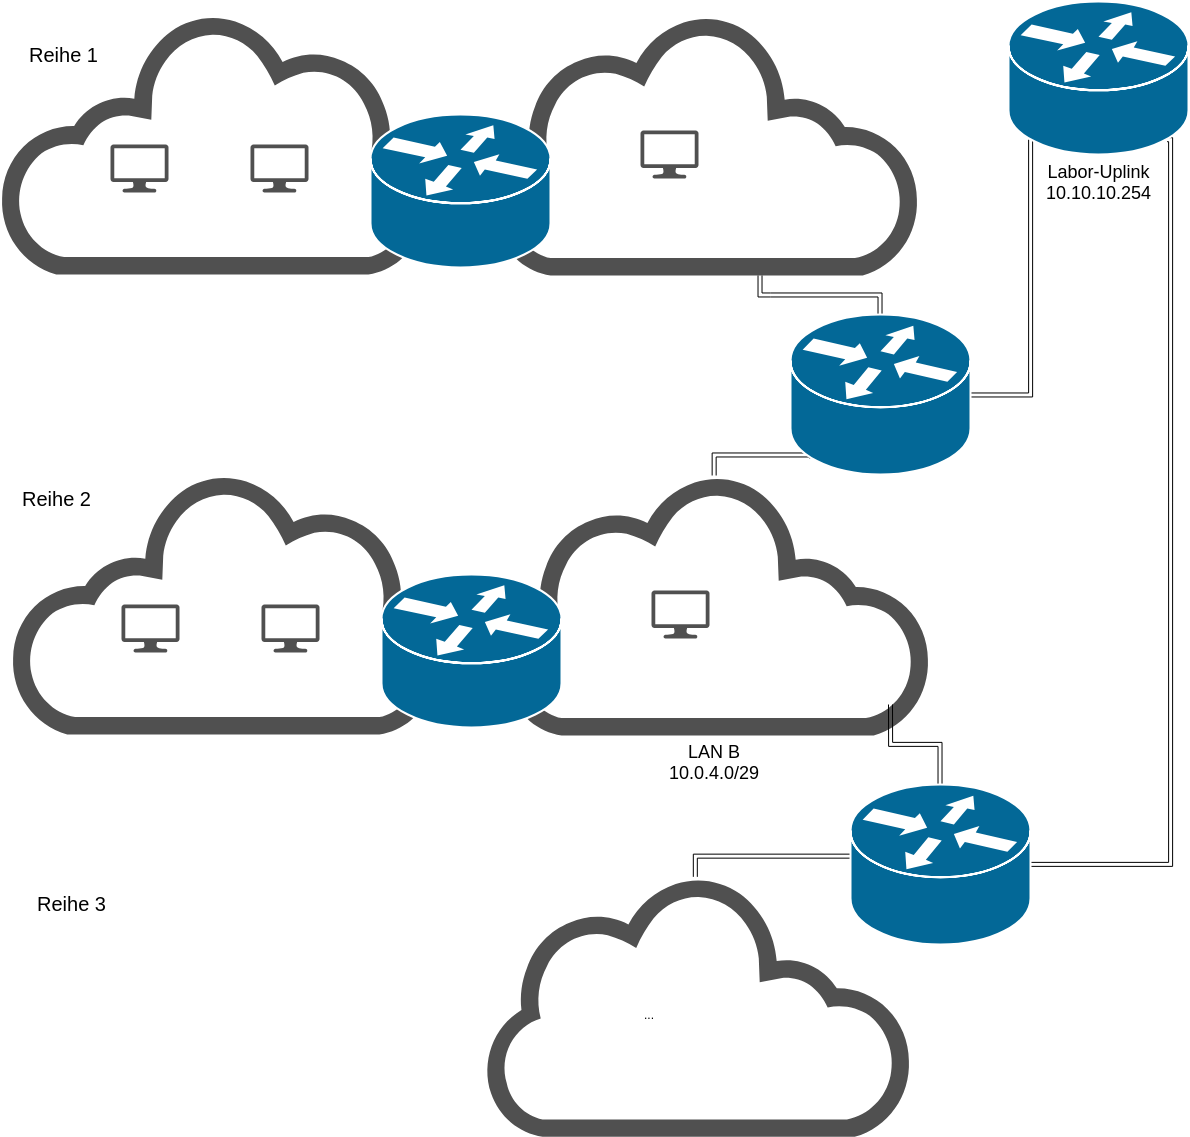
\includegraphics[scale=0.35]{backbone}
	\caption{Skizze des Netzwerkes bestehend aus fünf Bankreihen á zwei LANs, sowie den Backbone-Routern}
	\label{backbone}
	\end{figure}
Folgendes Adressschema gilt:
\begin{table}[H]
\caption{Adressschema für das Labor}
\label{adress_scheme}
\centering
\begin{tabular}{|c|c|}\hline
 & \textbf{IP  || IP-Range} \\ \hline
 $LAN_X$ & 10.0.$X$.Y/Size \\ \hline
 Backbone & 10.10.10.100 + $\rho$ \\ \hline
 Labornetz & 10.0.0.0/8 \\ \hline
 Uplink & 10.10.10.254 \\ \hline
 DNS & 10.10.10.254 \\ \hline
\end{tabular}
\end{table} 
$LAN_X$ bezeichnet die beiden Netzwerke der letzten Übung (Ihre Bankreihe mit je zwei Subnetzen), wobei der Wert $X$ der Reihe nach hochgezählt wird. D.h. Bankreihe eins: $LAN_{1}$, Bankreihe zwei: $LAN_{2}$ etc. Beachten Sie hierbei, dass Sie festlegen müssen wo ein Netzsegment beginnt und wo dies auch endet. 
\begin{tasks}
		\task~ Planen Sie entsprechend der Skizze Ihr Netzwerk. D.h. planen Sie entsprechende IP-Adressen, Subnetzmasken und Router ein.
		\task~ Skizzieren Sie Ihre lokalen Netzwerke, sowie das gesamte Netzwerk mitsamt der Router (Nutzen Sie geeignete Symbole).
		\task~ Planen Sie ebenso den Backbone-Router, sowie den Uplink (Router im Rack -- Zugang zum DFN(Internet) ein.
	\end{tasks}
	
\begin{center}\Large{\textbf{Aufgabe B -- Tools}}\end{center}\vskip0.25in
\begin{enumerate}
	\item Zwei weitere bekannte Netzwerkanalyse-Tools sind \emph{netstat} (\emph{net-tools}) und \emph{ss} aus der \emph{iproute2} Werkzeugsammlung.
\begin{tasks}
		\task~ Recherchieren Sie die wesentliche Funktionen von \emph{netstat}, sowie \emph{ss}.
		\task~ Notieren Sie sich anhand von Beispielen die Syntax der eben genannten Tools. 
	\end{tasks}
	\item \emph{iptables} sind unter Linux allgemein als Firewall-Tool bekannt. \footnote{Mehr zu Firewalling in der IT-Security Übung.} In der kommenden Übung übernimmt iptables eine etwas andere Aufgabe. Es sorgt zunächst dafür, dass unsere Raspberry Pis via \emph{NAT}\footnote{Um genau zu sein: SNAT} Pakte in das Internet routen können.
	\begin{tasks}
		\task~ Recherchieren Sie mithilfe folgenden Links was \emph{NAT} ist und warum dies unter \emph{IPv4} genutzt wird.\\
		\url{https://en.wikipedia.org/wiki/Network_address_translation}
		\task~ Machen Sie sich im groben klar, wie \emph{NAT} umgesetzt wird. 
		\task~ \textbf{Fakultativ:} Mit sehr hoher Wahrscheinlichkeit nutzt auch Ihr Router/Modem \emph{NAT}, wie wird dies hier umgesetzt?
		\task~ Recherchieren Sie was unter einer Firewall im wesentlichen verstanden wird.
		\task~ Machen Sie sich klar, wie dies im Groben vonstatten geht.
		\task~ \emph{iptables} kann genutzt werden, um die privaten Adressen auf öffentliche zu übersetzen. Lesen Sie folgenden Artikel:\\
		\url{https://access.redhat.com/documentation/en-US/Red_Hat_Enterprise_Linux/4/html/Security_Guide/s1-firewall-ipt-fwd.html}\\
		Versuchen Sie den Inhalt wirklich komplett zu verstehen. Notieren Sie sich alle notwendigen Schritte um das Masquerading via ip-tables einzuschalten.
		\task~ \emph{iptables} unterstützt sowohl \emph{SNAT} als auch \emph{DNAT}. Recherchieren Sie kurz worin sich beide Arten unterscheiden.
	\end{tasks}
\end{enumerate}
\begin{center}\Large{\textbf{Aufgabe C -- Routing \& Routing-Algorithmen}}\end{center}\vskip0.25in
In der letzten und in der kommenden Übung fällt ständig der ominöse Begriff Routing. Im wesentlichen haben Sie bereits in Erfahrung gebracht, was unter Routing zu verstehen ist. Als angehende Informatiker reicht jedoch kein oberflächliches Wissen, wenn Sie wirklich verstehen wollen, wie die Dinge funktionieren. Routing wird im wesentlichen durch zwei Routing-Algorithmen bewerkstelligt: dem Dijkstra- und dem Bellman-Ford-Algorithmus.
\begin{itemize}
	\item Recherchieren Sie zunächst was ein mathematischer Graph ist und wie Graphen im Kontext von Netzwerken genutzt werden können.
	\item Recherchieren Sie zunächst welche beiden Möglichen Ansätze (Link-State \& Distanzvektor) es gibt und worin sich diese fundamental unterscheiden.
	\item Finden Sie heraus, welches der beiden Verfahren aufgrund seiner Eigenschaften, für welchen Einsatz sinnvoll erscheint.
	\item Suchen Sie einigen einfachen Beispielen für den Dijkstra- und für den Bellman-Ford-Algorithmus. Verfolgen Sie anhand Ihrer gewählten Beispiele, wie das Routing funktioniert.
	\item Bringen Sie in Erfahrung welcher algorithmischer Ansatz in welchem Routing-Protokoll zum Einsatz kommt. Machen Sie sich klar, warum sich für welches Verfahren entschieden worden ist.
\end{itemize}
\begin{center}\Large{\textbf{Aufgabe D -- IPv6}}\end{center}\vskip0.25in
Im zweiten Übungsblatt haben Sie bereits eine kurzen Blick auf \emph{IPv6} geworfen. Momentan wird zwar immer noch vornehmlich auf das \glqq alte\grqq\ Internetprotokoll gesetzt, Sie jedoch sollen auch fit für die Zukunft sein.
\begin{enumerate}
	\item Rufen Sie sich erneut ins Gedächtnis welche Vorteile \emph{IPv6} mit sich bringt.
	\item Recherchieren Sie zunächst den Adressaufbau von \emph{IPv6}. Aus welchen Teilen besteht dies und welche Aufgabe/Zweck erfüllen die einzelnen Bestandteile.
	\item Machen Sie sich anschließend mit der Adressnotation vertraut! Notieren und kommentieren Sie einige Beispiele.
	\item Wie \emph{IPv4} hat auch \emph{IPv6} private Adressbereiche. Welche sind dies und wie ist deren Aufbau?
	\item Recherchieren Sie wie die \emph{CIDR}-Notation für \emph{IPv6} aussieht.
	\item Recherchieren Sie wie die Vergabe von \emph{IPv6}-Adressen und das setzen von \emph{IPv6} Routen aussieht. Machen Sie sich auch hier klar, was die einzelnen Bestandteile der Kommandos bewirken!
	\item Um das Routing zu ermöglichen benötigen Sie genau wie bei \emph{IPv4} eine Routing-Tabelle. Recherchieren Sie entsprechend, wie das Routing zu aktivieren ist.
\end{enumerate}

\end{document}